%%%%%%%%%%%%%%%%%%%%%%%%%%%%%%%%%%%%%%%%%
% Programming/Coding Assignment
% LaTeX Template
%
% This template has been downloaded from:
% http://www.latextemplates.com
%
% Original author:
% Ted Pavlic (http://www.tedpavlic.com)
%
% Note:
% The \lipsum[#] commands throughout this template generate dummy text
% to fill the template out. These commands should all be removed when 
% writing assignment content.
%
% This template uses a Perl script as an example snippet of code, most other
% languages are also usable. Configure them in the "CODE INCLUSION 
% CONFIGURATION" section.
%
%%%%%%%%%%%%%%%%%%%%%%%%%%%%%%%%%%%%%%%%%

%----------------------------------------------------------------------------------------
%	PACKAGES AND OTHER DOCUMENT CONFIGURATIONS
%----------------------------------------------------------------------------------------

\documentclass[a4paper]{article}

\usepackage{fancyhdr} % Required for custom headers
\usepackage{lastpage} % Required to determine the last page for the footer
\usepackage{extramarks} % Required for headers and footers
\usepackage[usenames,dvipsnames]{color} % Required for custom colors
\usepackage{graphicx} % Required to insert images
\usepackage{listings} % Required for insertion of code
\usepackage{courier} % Required for the courier font
\usepackage{lipsum} % Used for inserting dummy 'Lorem ipsum' text into the template
\usepackage{multirow}
\usepackage{tabu}
\usepackage{float}
\usepackage{pbox}
\usepackage{subcaption}

\usepackage{listings}
\usepackage{color}

\definecolor{dkgreen}{rgb}{0,0.6,0}
\definecolor{gray}{rgb}{0.5,0.5,0.5}
\definecolor{mauve}{rgb}{0.58,0,0.82}

\lstset{frame=tb,
  language=Matlab,
  aboveskip=3mm,
  belowskip=3mm,
  showstringspaces=false,
  columns=flexible,
  basicstyle={\small\ttfamily},
  numbers=none,
  numberstyle=\tiny\color{gray},
  keywordstyle=\color{blue},
  commentstyle=\color{dkgreen},
  stringstyle=\color{mauve},
  breaklines=true,
  breakatwhitespace=true
  tabsize=3
}

% Margins
\topmargin=-0.45in
\evensidemargin=0in
\oddsidemargin=0in
\textwidth=6.5in
\textheight=9.5in
\headsep=0.25in

\linespread{1.1} % Line spacing

% Set up the header and footer
\pagestyle{fancy}
\lhead{\hmwkAuthorName} % Top left header
\chead{\hmwkShortTitle} % Top center head
\rhead{\firstxmark} % Top right header
\lfoot{\lastxmark} % Bottom left footer
\cfoot{} % Bottom center footer
\rfoot{Page\ \thepage\ of\ \protect\pageref{LastPage}} % Bottom right footer
\renewcommand\headrulewidth{0.4pt} % Size of the header rule
\renewcommand\footrulewidth{0.4pt} % Size of the footer rule

\setlength\parindent{0pt} % Removes all indentation from paragraphs

%----------------------------------------------------------------------------------------
%	CODE INCLUSION CONFIGURATION
%----------------------------------------------------------------------------------------

\definecolor{MyDarkGreen}{rgb}{0.0,0.4,0.0} % This is the color used for comments
\lstloadlanguages{Matlab} % Load Perl syntax for listings, for a list of other languages supported see: ftp://ftp.tex.ac.uk/tex-archive/macros/latex/contrib/listings/listings.pdf
\lstset{language=Matlab, % Use Perl in this example
        frame=single, % Single frame around code
        basicstyle=\small\ttfamily, % Use small true type font
        keywordstyle=[1]\color{Blue}\bf, % Perl functions bold and blue
        keywordstyle=[2]\color{Purple}, % Perl function arguments purple
        keywordstyle=[3]\color{Blue}\underbar, % Custom functions underlined and blue
        identifierstyle=, % Nothing special about identifiers                                         
        commentstyle=\usefont{T1}{pcr}{m}{sl}\color{MyDarkGreen}\small, % Comments small dark green courier font
        stringstyle=\color{Purple}, % Strings are purple
        showstringspaces=false, % Don't put marks in string spaces
        tabsize=5, % 5 spaces per tab
        %
        % Put standard Perl functions not included in the default language here
        morekeywords={rand},
        %
        % Put Perl function parameters here
        morekeywords=[2]{on, off, interp},
        %
        % Put user defined functions here
        morekeywords=[3]{test},
       	%
        morecomment=[l][\color{Blue}]{...}, % Line continuation (...) like blue comment
        numbers=left, % Line numbers on left
        firstnumber=1, % Line numbers start with line 1
        numberstyle=\tiny\color{Blue}, % Line numbers are blue and small
        stepnumber=5 % Line numbers go in steps of 5
}

% Creates a new command to include a perl script, the first parameter is the filename of the script (without .pl), the second parameter is the caption
\newcommand{\matlabscript}[2]{
\begin{itemize}
\item[]\lstinputlisting[caption=#2,label=#1]{#1.m}
\end{itemize}
}

%----------------------------------------------------------------------------------------
%	DOCUMENT STRUCTURE COMMANDS
%	Skip this unless you know what you're doing
%----------------------------------------------------------------------------------------

% Header and footer for when a page split occurs within a problem environment
\newcommand{\enterProblemHeader}[1]{
\nobreak\extramarks{#1}{#1 continued on next page\ldots}\nobreak
\nobreak\extramarks{#1 (continued)}{#1 continued on next page\ldots}\nobreak
}

% Header and footer for when a page split occurs between problem environments
\newcommand{\exitProblemHeader}[1]{
\nobreak\extramarks{#1 (continued)}{#1 continued on next page\ldots}\nobreak
\nobreak\extramarks{#1}{}\nobreak
}

\setcounter{secnumdepth}{0} % Removes default section numbers
\newcounter{homeworkProblemCounter} % Creates a counter to keep track of the number of problems

\newcommand{\homeworkProblemName}{}
\newenvironment{homeworkProblem}[1][Problem \arabic{homeworkProblemCounter}]{ % Makes a new environment called homeworkProblem which takes 1 argument (custom name) but the default is "Problem #"
\stepcounter{homeworkProblemCounter} % Increase counter for number of problems
\renewcommand{\homeworkProblemName}{#1} % Assign \homeworkProblemName the name of the problem
\section{\homeworkProblemName} % Make a section in the document with the custom problem count
\enterProblemHeader{\homeworkProblemName} % Header and footer within the environment
}{
\exitProblemHeader{\homeworkProblemName} % Header and footer after the environment
}

\newcommand{\problemAnswer}[1]{ % Defines the problem answer command with the content as the only argument
\noindent\framebox[\columnwidth][c]{\begin{minipage}{0.98\columnwidth}#1\end{minipage}} % Makes the box around the problem answer and puts the content inside
}

\newcommand{\homeworkSectionName}{}
\newenvironment{homeworkSection}[1]{ % New environment for sections within homework problems, takes 1 argument - the name of the section
\renewcommand{\homeworkSectionName}{#1} % Assign \homeworkSectionName to the name of the section from the environment argument
\subsection{\homeworkSectionName} % Make a subsection with the custom name of the subsection
\enterProblemHeader{\homeworkProblemName\ [\homeworkSectionName]} % Header and footer within the environment
}{
\enterProblemHeader{\homeworkProblemName} % Header and footer after the environment
}

%----------------------------------------------------------------------------------------
%	NAME AND CLASS SECTION
%----------------------------------------------------------------------------------------

\newcommand{\hmwkTitle}{CO395 Machine Learning\\CBC \#2\\Artificial Neural Networks} % Assignment title
\newcommand{\hmwkShortTitle}{CBC \#2 - Artificial Neural Networks}
\newcommand{\hmwkDueDate}{Monday,\ November\ 4,\ 2013} % Due date
\newcommand{\hmwkAuthorName}{Group 1} % Your name

%----------------------------------------------------------------------------------------
%	TITLE PAGE
%----------------------------------------------------------------------------------------

\title{
\vspace{2in}
\textmd{\textbf{\hmwkTitle}}\\
%\normalsize\vspace{0.1in}\small{Due\ on\ \hmwkDueDate}\\
%\vspace{0.1in}\large{\textit{\hmwkClassInstructor\ \hmwkClassTime}}
\vspace{3in}
\textbf{Group 1}\\
Yong Wen Chua, \texttt{ywc110}\\
Thomas Morrison, \texttt{tm1810}\\
Marcin Baginski, \texttt{mgb10}\\
Marcin Kadziela, \texttt{mk4910}
}

%\author{\textbf{\hmwkAuthorName}}

\date{} % Insert date here if you want it to appear below your name

%----------------------------------------------------------------------------------------

\begin{document}

\maketitle

%----------------------------------------------------------------------------------------
%	TABLE OF CONTENTS
%----------------------------------------------------------------------------------------

%\setcounter{tocdepth}{1} % Uncomment this line if you don't want subsections listed in the ToC

\newpage
\tableofcontents
\newpage

%----------------------------------------------------------------------------------------
%	SECTION 1 - Implementation Details
%----------------------------------------------------------------------------------------

\section{Implementation Details}
\subsection{Overview}
This report describes the work conducted in the second assignment of the Machine Learning course. The main goal of this coursework was to investigate and learn how to use MATLAB's Neural Network Toolbox. The task that we were given was a typical pattern recognition and classification problem. We were supposed to train, test and evaluate one network with multiple outputs and multiple single-output neural networks (one for each class). We started this assignment by optimising parameters for each of these networks. The approach taken was optimising topology together with the training function first. In later phases we focused on other parameters (such as minimum gradient or goal) which could reduce the problem of overfitting. Eventually, we used the 10-fold cross-validation in order to compare the performance of the two network types.

\subsection{Description of the MATLAB functions}
\begin{itemize}
\item \texttt{nFoldValidate(examples, classifications, n, networkType)} - performs the n-fold cross-validation. Takes as arguments the examples, classifications, number of folds and the network type (\texttt{'single'} or \texttt{'multi'}). Based on the network type, it either generates multiple single-output networks or one multi-output network and validates them. It returns a cell array which contains the confusion matrices for each fold
\item \texttt{generateMultiOutputNetwork(xANN, yANN, layers, neurons, transferFcn,\\trainingFcn, lr, grad, goal)} - generates a multiple-output network based on the arguments which are passed to the function. These include the number of layers, neurons in a layer, training function, transfer function, learning rate, stopping gradient and the performance goal. It is used within \texttt{nFoldValidate()}
\item \texttt{generateSingleOutputNetworks(xANN, yANN, layers, neurons, transferFcn,\\trainingFcn, lr, grad, goal)} - generates multiple single-output networks based on the same arguments as the previous function
\item \texttt{testANN(network, inputs)} - produces a vector of predictions for the  inputs using provided neural network (either the multi or single output one)
\item \texttt{recallPrecisionF1(confusionMatrix)} - calculates the recall, precision and $F_1$ measures after taking the confusion matrix as an argument
\item \texttt{plotAverageF1Measure(confusionMatrixSingle, confusionMatrixMulti)} - takes two arrays of confusion matrices (one for each fold) from the single and multi-output networks and plots the average F1 measure for each fold. Its output is a direct answer to the question from Part VIII
\item \texttt{confusion\_matrix(actual, predicted, possible\_outcomes)} - calculates the confusion matrix given a column vector of actual and predicted outcomes
\end{itemize}

\clearpage

%----------------------------------------------------------------------------------------
%	SECTION 2 - Evaluation
%----------------------------------------------------------------------------------------

\section{Evaluation}
The average $F_1$ measure per fold for both types of networks is presented below:
\begin{figure}[H]
\center
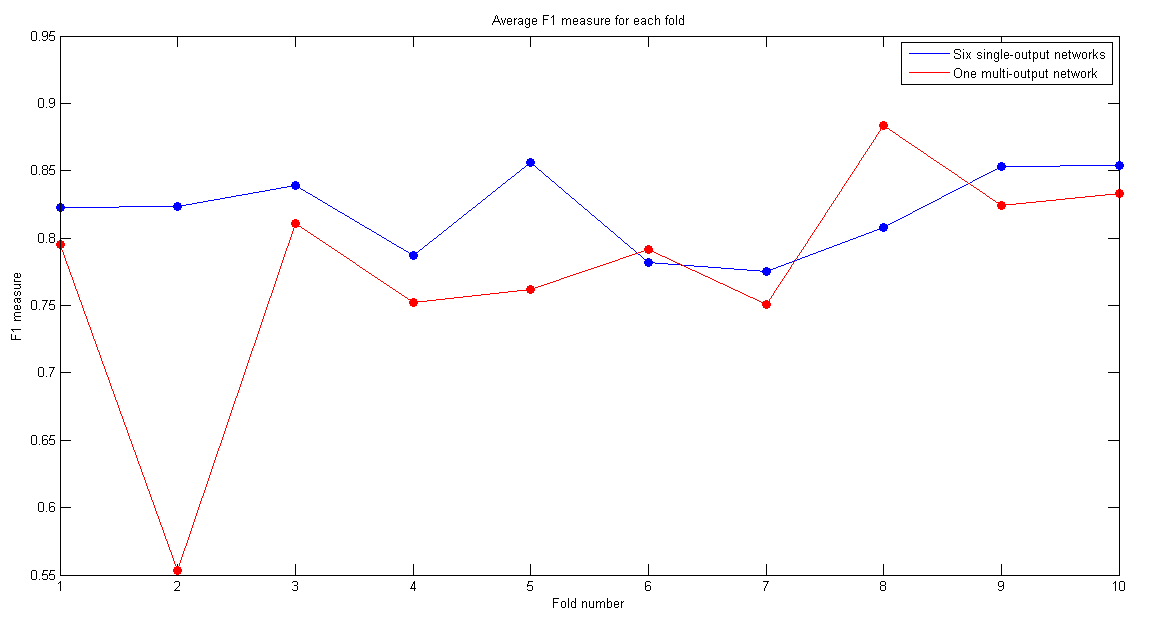
\includegraphics[width=0.9\columnwidth]{averageF1eachFold}
\caption{Average $F_1$ measure per fold for both types of networks}
\end{figure}

\subsection{Clean dataset}
\subsubsection{Single six-output network}

\begin{table}[H]
\center
\begin{tabu}{cc|c|c|c|c|c|c|}
\cline{3-8}
& & \multicolumn{6}{ c| }{Predicted class} \\ \cline{3-8}
& & 1 & 2 & 3 & 4 & 5 & 6 \\ \cline{1-2} \tabucline[1.5pt]{3-8}
\multicolumn{1}{ |c| }{\multirow{6}{*}{Actual class} } &
\multicolumn{1}{ |c|[1.5pt] }{1} & \textbf{86} & 18 & 6 & 6 & 14 & 2 \\ \cline{2-8}
\multicolumn{1}{ |c| }{}                        &
\multicolumn{1}{ |c|[1.5pt] }{2} & 9 & \textbf{167} & 6 & 5 & 11 & 0 \\ \cline{2-8}
\multicolumn{1}{ |c|  }{}                        &
\multicolumn{1}{ |c|[1.5pt] }{3} & 2 & 5 & \textbf{97} & 3 & 5 & 7 \\ \cline{2-8}
\multicolumn{1}{ |c|  }{}                        &
\multicolumn{1}{ |c|[1.5pt] }{4} & 0 & 6 & 1 & \textbf{203} & 4 & 2 \\ \cline{2-8}
\multicolumn{1}{ |c|  }{}                        &
\multicolumn{1}{ |c|[1.5pt] }{5} & 7 & 26 & 2 & 3 & \textbf{92} & 2 \\ \cline{2-8}
\multicolumn{1}{ |c|  }{}                        &
\multicolumn{1}{ |c|[1.5pt] }{6} & 0 & 3 & 12 & 2 & 2 & \textbf{188} \\ \cline{1-8}
\end{tabu}
\caption{Confusion Matrix for single six-output ANN for the \emph{clean} dataset}
\label{confusionMatrixCleanSixOutput}
\end{table}

\begin{table}[H]
\center
\begin{tabu}{cc|c|c|c|}
\cline{3-5}
& & Recall & Precision & $F_1$ \\ \cline{1-2} \tabucline[1.5pt]{3-5}
\multicolumn{1}{ |c| }{\multirow{6}{*}{Actual class} } &
\multicolumn{1}{ |c|[1.5pt] }{1} & 65\% & 83\% & 73\% \\ \cline{2-5}
\multicolumn{1}{ |c| }{}                        &
\multicolumn{1}{ |c|[1.5pt] }{2} & 84\% & 74\% & 79\% \\ \cline{2-5}
\multicolumn{1}{ |c|  }{}                        &
\multicolumn{1}{ |c|[1.5pt] }{3} & 82\% & 78\% & 80\% \\ \cline{2-5}
\multicolumn{1}{ |c|  }{}                        &
\multicolumn{1}{ |c|[1.5pt] }{4} & 94\% & 91\% & 93\% \\ \cline{2-5}
\multicolumn{1}{ |c|  }{}                        &
\multicolumn{1}{ |c|[1.5pt] }{5} & 70\% & 72\% & 71\% \\ \cline{2-5}
\multicolumn{1}{ |c|  }{}                        &
\multicolumn{1}{ |c|[1.5pt] }{6} & 91\% & 94\% & 92\% \\ \cline{1-5}
\end{tabu}
\caption{Recall, precision and $F_1$ measure for single six-output ANN for the \emph{clean} dataset}
\label{recallPrecisionF1CleanCleanSixOutput}
\end{table}

\begin{figure}[H]
\[ C = \frac{833}{1004} = 83.0\% \]
\caption{Classification rate for single six-output ANN for the \emph{clean} dataset}
\end{figure}

\subsubsection{Six single-output networks}

\begin{table}[H]
\center
\begin{tabu}{cc|c|c|c|c|c|c|}
\cline{3-8}
& & \multicolumn{6}{ c| }{Predicted class} \\ \cline{3-8}
& & 1 & 2 & 3 & 4 & 5 & 6 \\ \cline{1-2} \tabucline[1.5pt]{3-8}
\multicolumn{1}{ |c| }{\multirow{6}{*}{Actual class} } &
\multicolumn{1}{ |c|[1.5pt] }{1} & \textbf{99} & 12 & 7 & 3 & 10 & 1 \\ \cline{2-8}
\multicolumn{1}{ |c| }{}                        &
\multicolumn{1}{ |c|[1.5pt] }{2} & 9 & \textbf{168} & 3 & 6 & 11 & 1 \\ \cline{2-8}
\multicolumn{1}{ |c|  }{}                        &
\multicolumn{1}{ |c|[1.5pt] }{3} & 4 & 2 & \textbf{98} & 2 & 3 & 10 \\ \cline{2-8}
\multicolumn{1}{ |c|  }{}                        &
\multicolumn{1}{ |c|[1.5pt] }{4} & 2 & 4 & 2 & \textbf{205} & 1 & 2 \\ \cline{2-8}
\multicolumn{1}{ |c|  }{}                        &
\multicolumn{1}{ |c|[1.5pt] }{5} & 8 & 21 & 7 & 4 & \textbf{89} & 3 \\ \cline{2-8}
\multicolumn{1}{ |c|  }{}                        &
\multicolumn{1}{ |c|[1.5pt] }{6} & 0 & 3 & 10 & 5 & 2 & \textbf{187} \\ \cline{1-8}
\end{tabu}
\caption{Confusion Matrix for six single-output ANNs for the \emph{clean} dataset}
\label{confusionMatrixCleanSingleOutput}
\end{table}

\begin{table}[H]
\center
\begin{tabu}{cc|c|c|c|}
\cline{3-5}
& & Recall & Precision & $F_1$ \\ \cline{1-2} \tabucline[1.5pt]{3-5}
\multicolumn{1}{ |c| }{\multirow{6}{*}{Actual class} } &
\multicolumn{1}{ |c|[1.5pt] }{1} & 75\% & 81\% & 78\% \\ \cline{2-5}
\multicolumn{1}{ |c| }{}                        &
\multicolumn{1}{ |c|[1.5pt] }{2} & 84\% & 80\% & 82\% \\ \cline{2-5}
\multicolumn{1}{ |c|  }{}                        &
\multicolumn{1}{ |c|[1.5pt] }{3} & 82\% & 77\% & 80\% \\ \cline{2-5}
\multicolumn{1}{ |c|  }{}                        &
\multicolumn{1}{ |c|[1.5pt] }{4} & 95\% & 91\% & 93\% \\ \cline{2-5}
\multicolumn{1}{ |c|  }{}                        &
\multicolumn{1}{ |c|[1.5pt] }{5} & 67\% & 77\% & 72\% \\ \cline{2-5}
\multicolumn{1}{ |c|  }{}                        &
\multicolumn{1}{ |c|[1.5pt] }{6} & 90\% & 92\% & 91\% \\ \cline{1-5}
\end{tabu}
\caption{Recall, precision and $F_1$ measure for six single-output ANNs for the \emph{clean} dataset}
\label{recallPrecisionF1CleanCleanSingleOutput}
\end{table}

\begin{figure}[H]
\[ C = \frac{846}{1004} = 84.3\% \]
\caption{Classification rate for six single-output ANNs for the \emph{clean} dataset}
\end{figure}

\subsection{Noisy dataset}

\subsubsection{Single six-output network}

\begin{table}[H]
\center
\begin{tabu}{cc|c|c|c|c|c|c|}
\cline{3-8}
& & \multicolumn{6}{ c| }{Predicted class} \\ \cline{3-8}
& & 1 & 2 & 3 & 4 & 5 & 6 \\ \cline{1-2} \tabucline[1.5pt]{3-8}
\multicolumn{1}{ |c| }{\multirow{6}{*}{Actual class} } &
\multicolumn{1}{ |c|[1.5pt] }{1} & \textbf{11} & 16 & 22 & 7 & 25 & 7 \\ \cline{2-8}
\multicolumn{1}{ |c| }{}                        &
\multicolumn{1}{ |c|[1.5pt] }{2} & 4 & \textbf{149} & 18 & 6 & 6 & 4 \\ \cline{2-8}
\multicolumn{1}{ |c|  }{}                        &
\multicolumn{1}{ |c|[1.5pt] }{3} & 2 & 15 & \textbf{132} & 10 & 9 & 19 \\ \cline{2-8}
\multicolumn{1}{ |c|  }{}                        &
\multicolumn{1}{ |c|[1.5pt] }{4} & 3 & 7 & 13 & \textbf{175} & 4 & 7 \\ \cline{2-8}
\multicolumn{1}{ |c|  }{}                        &
\multicolumn{1}{ |c|[1.5pt] }{5} & 7 & 13 & 14 & 5 & \textbf{56} & 15 \\ \cline{2-8}
\multicolumn{1}{ |c|  }{}                        &
\multicolumn{1}{ |c|[1.5pt] }{6} & 1 & 4 & 15 & 5 & 9 & \textbf{186} \\ \cline{1-8}
\end{tabu}
\caption{Confusion Matrix for single six-output ANN for the \emph{noisy} dataset}
\label{confusionMatrixNoisySixOutput}
\end{table}

\begin{table}[H]
\center
\begin{tabu}{cc|c|c|c|}
\cline{3-5}
& & Recall & Precision & $F_1$ \\ \cline{1-2} \tabucline[1.5pt]{3-5}
\multicolumn{1}{ |c| }{\multirow{6}{*}{Actual class} } &
\multicolumn{1}{ |c|[1.5pt] }{1} & 13\% & 39\% & 19\% \\ \cline{2-5}
\multicolumn{1}{ |c| }{}                        &
\multicolumn{1}{ |c|[1.5pt] }{2} & 80\% & 73\% & 76\% \\ \cline{2-5}
\multicolumn{1}{ |c|  }{}                        &
\multicolumn{1}{ |c|[1.5pt] }{3} & 71\% & 62\% & 66\% \\ \cline{2-5}
\multicolumn{1}{ |c|  }{}                        &
\multicolumn{1}{ |c|[1.5pt] }{4} & 84\% & 84\% & 84\% \\ \cline{2-5}
\multicolumn{1}{ |c|  }{}                        &
\multicolumn{1}{ |c|[1.5pt] }{5} & 51\% & 51\% & 51\% \\ \cline{2-5}
\multicolumn{1}{ |c|  }{}                        &
\multicolumn{1}{ |c|[1.5pt] }{6} & 85\% & 78\% & 81\% \\ \cline{1-5}
\end{tabu}
\caption{Recall, precision and $F_1$ measure for single six-output ANN for the \emph{noisy} dataset}
\label{recallPrecisionF1CleanNoisySixOutput}
\end{table}

\begin{figure}[H]
\[ C = \frac{709}{1001} = 70.8\% \]
\caption{Classification rate for single six-output ANN for the \emph{noisy} dataset}
\end{figure}

\subsubsection{Six single-output networks}

\begin{table}[H]
\center
\begin{tabu}{cc|c|c|c|c|c|c|}
\cline{3-8}
& & \multicolumn{6}{ c| }{Predicted class} \\ \cline{3-8}
& & 1 & 2 & 3 & 4 & 5 & 6 \\ \cline{1-2} \tabucline[1.5pt]{3-8}
\multicolumn{1}{ |c| }{\multirow{6}{*}{Actual class} } &
\multicolumn{1}{ |c|[1.5pt] }{1} & \textbf{15} & 11 & 25 & 8 & 23 & 6 \\ \cline{2-8}
\multicolumn{1}{ |c| }{}                        &
\multicolumn{1}{ |c|[1.5pt] }{2} & 3 & \textbf{154} & 15 & 6 & 7 & 2 \\ \cline{2-8}
\multicolumn{1}{ |c|  }{}                        &
\multicolumn{1}{ |c|[1.5pt] }{3} & 1 & 11 & \textbf{139} & 8 & 11 & 17 \\ \cline{2-8}
\multicolumn{1}{ |c|  }{}                        &
\multicolumn{1}{ |c|[1.5pt] }{4} & 1 & 9 & 11 & \textbf{176} & 6 & 6 \\ \cline{2-8}
\multicolumn{1}{ |c|  }{}                        &
\multicolumn{1}{ |c|[1.5pt] }{5} & 4 & 8 & 19 & 4 & \textbf{67} & 8 \\ \cline{2-8}
\multicolumn{1}{ |c|  }{}                        &
\multicolumn{1}{ |c|[1.5pt] }{6} & 1 & 3 & 13 & 4 & 9 & \textbf{190} \\ \cline{1-8}
\end{tabu}
\caption{Confusion Matrix for six single-output ANNs for the \emph{noisy} dataset}
\label{confusionMatrixNoisySingleOutput}
\end{table}

\begin{table}[H]
\center
\begin{tabu}{cc|c|c|c|}
\cline{3-5}
& & Recall & Precision & $F_1$ \\ \cline{1-2} \tabucline[1.5pt]{3-5}
\multicolumn{1}{ |c| }{\multirow{6}{*}{Actual class} } &
\multicolumn{1}{ |c|[1.5pt] }{1} & 17\% & 60\% & 27\% \\ \cline{2-5}
\multicolumn{1}{ |c| }{}                        &
\multicolumn{1}{ |c|[1.5pt] }{2} & 82\% & 79\% & 80\% \\ \cline{2-5}
\multicolumn{1}{ |c|  }{}                        &
\multicolumn{1}{ |c|[1.5pt] }{3} & 74\% & 63\% & 68\% \\ \cline{2-5}
\multicolumn{1}{ |c|  }{}                        &
\multicolumn{1}{ |c|[1.5pt] }{4} & 84\% & 85\% & 85\% \\ \cline{2-5}
\multicolumn{1}{ |c|  }{}                        &
\multicolumn{1}{ |c|[1.5pt] }{5} & 61\% & 54\% & 58\% \\ \cline{2-5}
\multicolumn{1}{ |c|  }{}                        &
\multicolumn{1}{ |c|[1.5pt] }{6} & 86\% & 83\% & 85\% \\ \cline{1-5}
\end{tabu}
\caption{Recall, precision and $F_1$ measure for six single-output ANNs for the \emph{noisy} dataset}
\label{recallPrecisionF1CleanNoisySingleOutput}
\end{table}

\begin{figure}[H]
\[ C = \frac{741}{1001} = 74.0\% \]
\caption{Classification rate for six single-output ANNs for the \emph{noisy} dataset}
\end{figure}

\clearpage
\subsection{Discussion of results}
Overall, we can say that our neural networks perform quite well, especially on the \emph{clean} dataset. There is one emotion in the \emph{noisy} dataset however, for which the performance is unsatisfactory - emotion 1 with $17\%$ recall and $60\%$ precision for the six single-output networks. It is also worth noting, that the neural networks perform better than the decision trees on both \emph{clean} and \emph{noisy} datasets. The best classification rate for the \emph{clean} dataset achieved by the decision trees was $74.0\%$ compared to $84.3\%$ scored by the neural networks. Similarly, for the \emph{noisy} dataset the results were $61.9\%$ compared to $74.0\%$.

\clearpage

%----------------------------------------------------------------------------------------
%	SECTION 3 - Questions
%----------------------------------------------------------------------------------------

\section{Questions}
\subsection{Optimal topology}
The final, optimal parameters for the two types of networks are:
\begin{enumerate}
\item Single six-output network:
\begin{itemize}
\item Hidden layers: 1
\item Hidden neurons: 23
\item Transfer function: \texttt{'tansig'} (sigmoid)
\item Training function: \texttt{'trainscg'}
\item Learning rate: 0.01
\item Minimum gradient: $3*10^{-6}$
\item Goal: $2*10^{-3}$
\end{itemize}
\item Six single-output networks:
\begin{itemize}
\item Hidden layers: 1
\item Hidden neurons: 9
\item Transfer function: \texttt{'tansig'} (sigmoid)
\item Training function: \texttt{'trainscg'}
\item Learning rate: 0.01
\item Minimum gradient: $5*10^{-6}$
\item Goal: $3*10^{-3}$
\end{itemize}
\end{enumerate}
We arrived at these values by performing a series of simulations of the performance of networks with different values on the first fold on the \emph{clean} dataset. In the first experiment, we tried to optimise the topology i.e. number of hidden layers, number of hidden neurons in each layer as well as the training function. We did this by repeatedly training the network with different parameters and plotted the results which are presented in \textbf{Figures \ref{multiOutput1layer}, \ref{multiOutput2layer}, \ref{singleOutput1layer}, \ref{singleOutput2layer}}. From the analysis of the results it can be concluded that the networks with just one hidden layer perform slightly better than those with two hidden layers, and so we trained our final networks with a single hidden layer. In case of the single six-output network, the peak is achieved for 32 hidden neurons, however as our final topology we selected 23 hidden neurons, since the classification rate for this topology is insignificantly smaller, yet the number of neurons is reduced by almost a third. For the six single-output networks, we decided to choose 9 hidden neurons. \medskip

In terms of the training function, it looks that \texttt{'trainscg'} and \texttt{'trainrp'} perform similarly, while \texttt{'trainlm'} almost always exhibits the worst performance. Due to the speed of training and the classification rates at our chosen numbers of hidden neurons, we ultimately choose \texttt{'trainscg'} as our training function for both types of networks. We also tried to look at the performance of \texttt{'trainbr'} function, however its running time was extremely slow and we ended up not including it. \medskip

We selected these values because we needed eventually to decide on the topology of the network. However, by looking at the plots, it is clear that the number of hidden layers and neurons (at least for the range of values which we investigated) does not cause the performance to vary significantly beyond some minimum number of neurons and before some maximum. As long as the number of hidden neurons is in some reasonable range (above 20 for the single six-output network and between 6 and 30 for six single-output networks), it does not matter themendously what exact value we would choose.

\begin{figure}[H]
\center
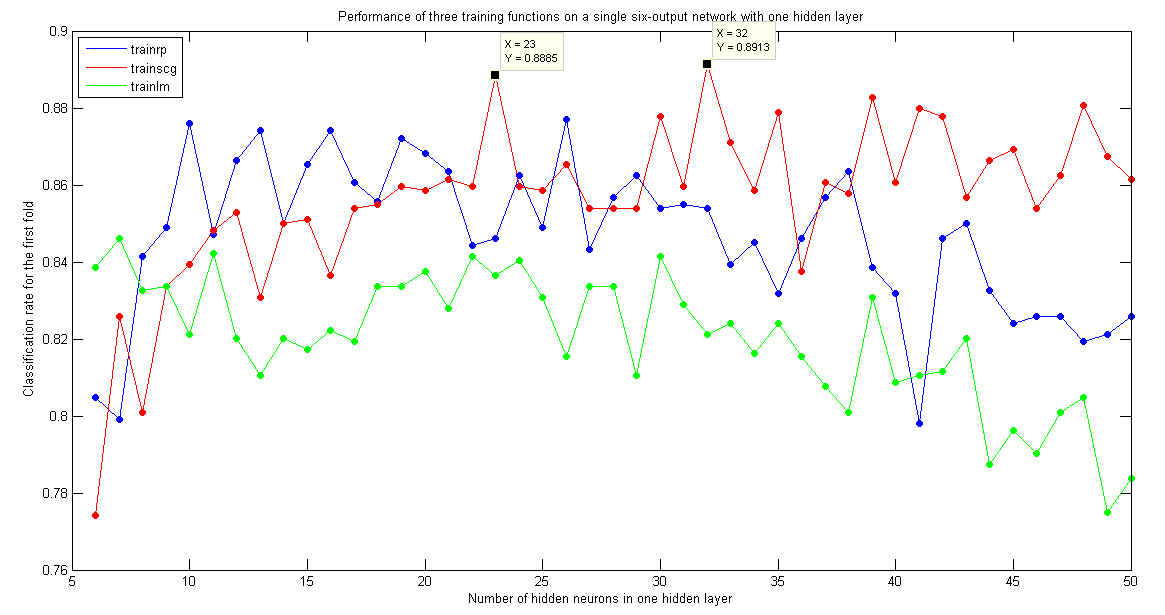
\includegraphics[width=1\columnwidth]{multiOutput1layer}
\caption{Classification rate for the first fold of the \emph{clean} dataset with respect to the training function and the number of hidden neurons for a single six-output network with one hidden layer}
\label{multiOutput1layer}
\end{figure}

\begin{figure}[H]
\center
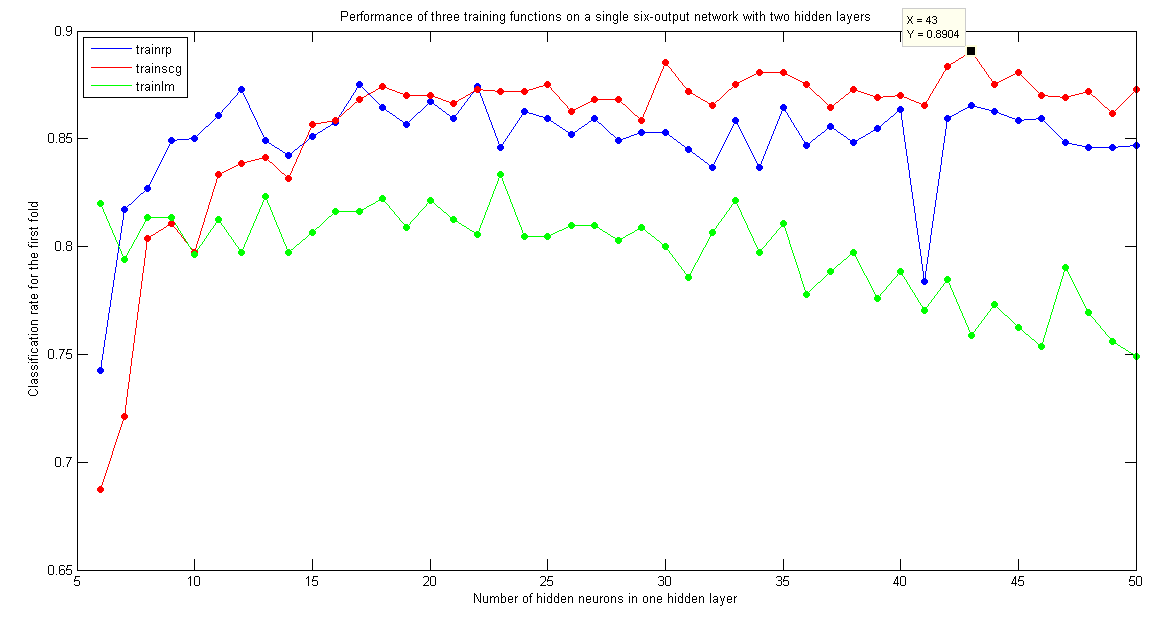
\includegraphics[width=1\columnwidth]{multiOutput2layer}
\caption{Classification rate for the first fold of the \emph{clean} dataset with respect to the training function and the number of hidden neurons for a single six-output network with two hidden layers}
\label{multiOutput2layer}
\end{figure}

\begin{figure}[H]
\center
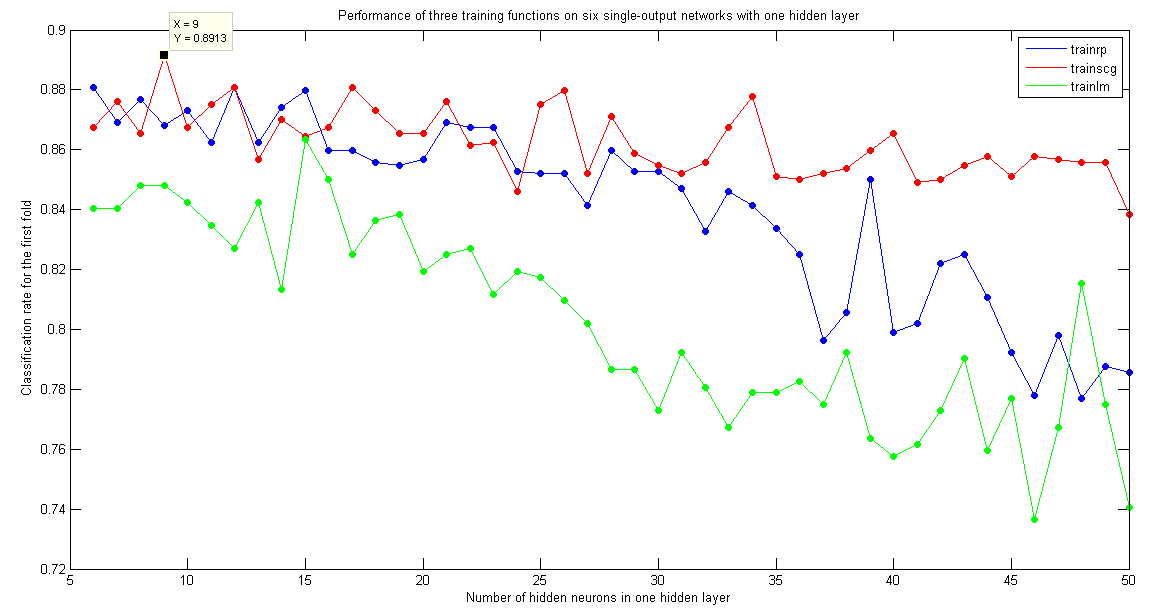
\includegraphics[width=1\columnwidth]{singleOutput1layer}
\caption{Classification rate for the first fold of the \emph{clean} dataset with respect to the training function and the number of hidden neurons for six single-output networks with one hidden layer}
\label{singleOutput1layer}
\end{figure}

\begin{figure}[H]
\center
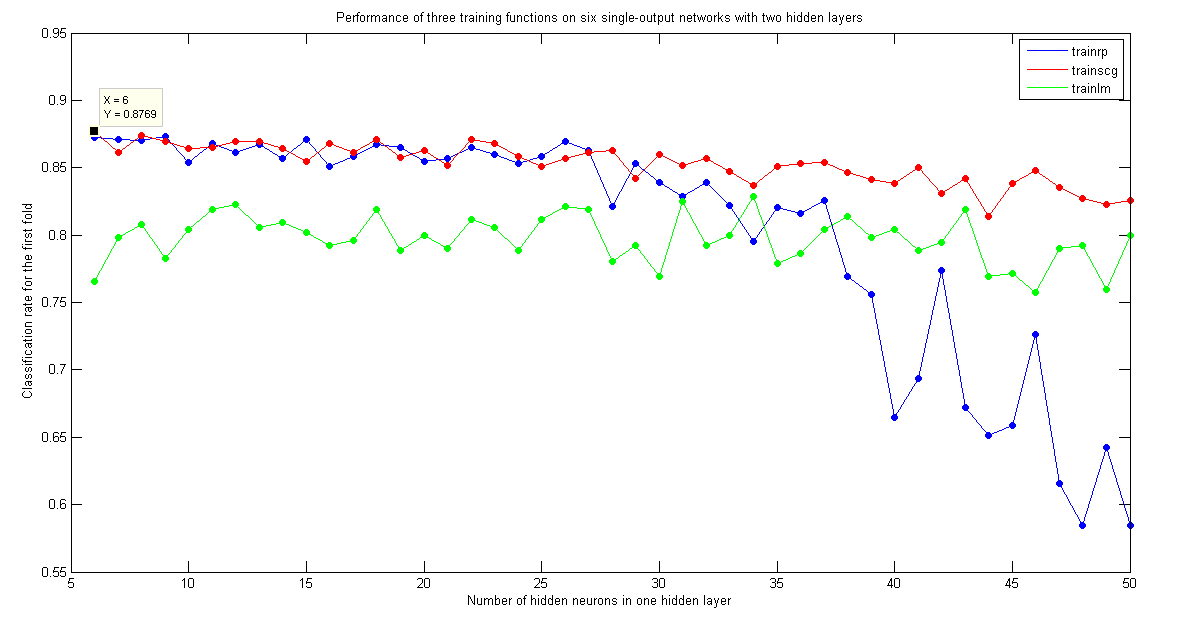
\includegraphics[width=1\columnwidth]{singleOutput2layer}
\caption{Classification rate for the first fold of the \emph{clean} dataset with respect to the training function and the number of hidden neurons for six single-output networks with two hidden layers}
\label{singleOutput2layer}
\end{figure}

\clearpage

\subsection{Overfitting}

There are several ways of avoid overfitting and therefore improve generalisation. General recommendation is to train network which is just large enough to provide a good fit. As mentioned in the book 'Pattern Recognition', excessive training on multi-layer network may result in poor generalisation 'as the net implements a complex decision boundary "tuned" to the specific training data'. In our experiment we focussed on networks which were as small as possible. \medskip

Another way to avoid overfitting is regularisation, which involves modifying performance function. Default performance function for \texttt{'trainscg'} was mean squared error. We noticed that by changing our function to the mean squared error and the mean squared weight and bias \texttt{'msereg'} we were able get results, which gave us higher classification rate, up to 1\%. In order to further improve our results we decided to work on early stopping. This was done by experimenting with the goal and minimum gradient. We ran simulations for both types of networks during which we varied the two parameters and the results of these simulations are presented in Figures \ref{singleOverfitting} and \ref{multiOverfitting}. It follows directly from the Figures that the optimal goal and minimum gradient for the six-output network are $2*10^{-3}$ and $3*10^{-6}$ respectively. For the six single-output networks it is $3*10^{-3}$ and $5*10^{-6}$.

\begin{figure}[!ht]
\centering
\begin{minipage}{.5\textwidth}
  \centering
  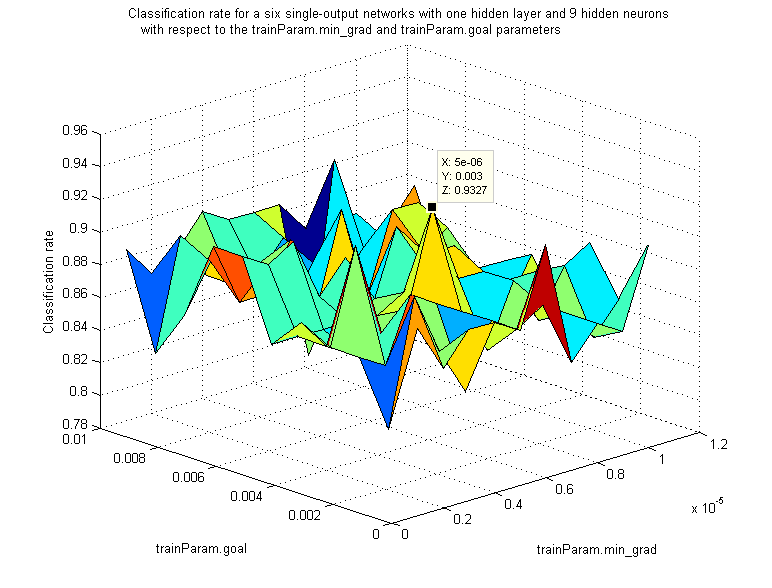
\includegraphics[width=1\linewidth]{singleOverfitting}
  \captionof{figure}{Classification rate for the first fold\\of the \emph{clean} dataset with respect to the minimum\\gradient and the performance goal for six single-\\output networks with the optimal topology\\outlined before}
  \label{singleOverfitting}
\end{minipage}%
\begin{minipage}{.5\textwidth}
  \centering
  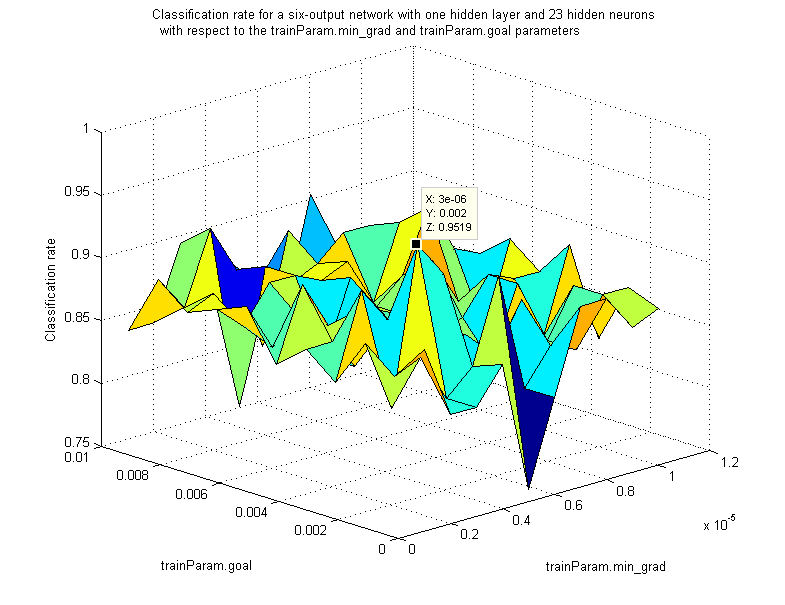
\includegraphics[width=1\linewidth]{multiOverfitting}
  \captionof{figure}{Classification rate for the first fold\\of the \emph{clean} dataset with respect to the minimum\\gradient and the performance goal for a single six-\\output network with the optimal topology\\outlined before}
  \label{multiOverfitting}
\end{minipage}
\end{figure}

\subsection{Six-output vs. single-output networks}
The aggregated classification rate for the both types of networks is presented in Table \ref{comparisonTable}.

\begin{table}[H]
\center
\begin{tabular}{c|c|c|}
\cline{2-3}
 & \pbox{20cm}{Classification rate \\ \emph{clean} dataset} & \pbox{20cm}{Classification rate \\ \emph{noisy} dataset} \\ \hline
\multicolumn{1}{ |c| }{Single six-output network} & 83.0\% & 70.8\% \\ \hline
\multicolumn{1}{ |c| }{Six single-output networks} & \textbf{84.3\%} & \textbf{74.0\%} \\ \hline
\end{tabular}
\caption{Aggregated classification rates for all strategies. Highlighted is the best result for a given dataset.}
\label{comparisonTable}
\end{table}

Clearly, the six single-output networks perform better in case of both datasets, however their advantage is not tremendous. This can be explained by the fact that six separate networks can be trained more specifically to detect one particular emotion than one six-output network. Just like in the real world, a General Practitioner can probably diagnose most common illnesses, yet six different specialist doctors might achieve a smaller misdiagnosis rate. Additionally, six single-output networks can be more robust to noise, since during training, noise appearing in the emotions which the network is not concerned with have smaller effect (the class associated with them is always 0). \medskip

The main advantage of the single-output networks is therefore improved classification rate. Their disadvantages include a slower performance and slower training as well as the possibility of two networks classifying the same example as two different emotions. In our case, since we are using the sigmoid as the transfer function, in order to break tie we always selected the network with greatest output. Similarly, the single six-output network's main advantage is its speed which comes at the expense of the average classification rate.

\subsection{Ideal parameter optimisation}

We believe that for the n-fold cross-validation the parameters should be optimised for each fold separately. For every set of parameters and fold we should also record the performance measure. Then, the ideal way would be to choose a set of parameters which result in the largest average classification rate across all folds. \medskip

Another good way to optimise the parameters for the network trained on the entire \emph{clean} dataset would be to discard the n-fold validation, and instead optimise the parameters on a single partition into training examples (probably around 900) and validation (the remaining examples). We do not need the test examples in this case, since all unseen data serves as such (including the one on which the network will be tested while marking this assignment).

\clearpage

%----------------------------------------------------------------------------------------
%	SECTION 4 - Code flowchart
%----------------------------------------------------------------------------------------

\section{Code Flowchart}

\begin{figure}[H]
\center
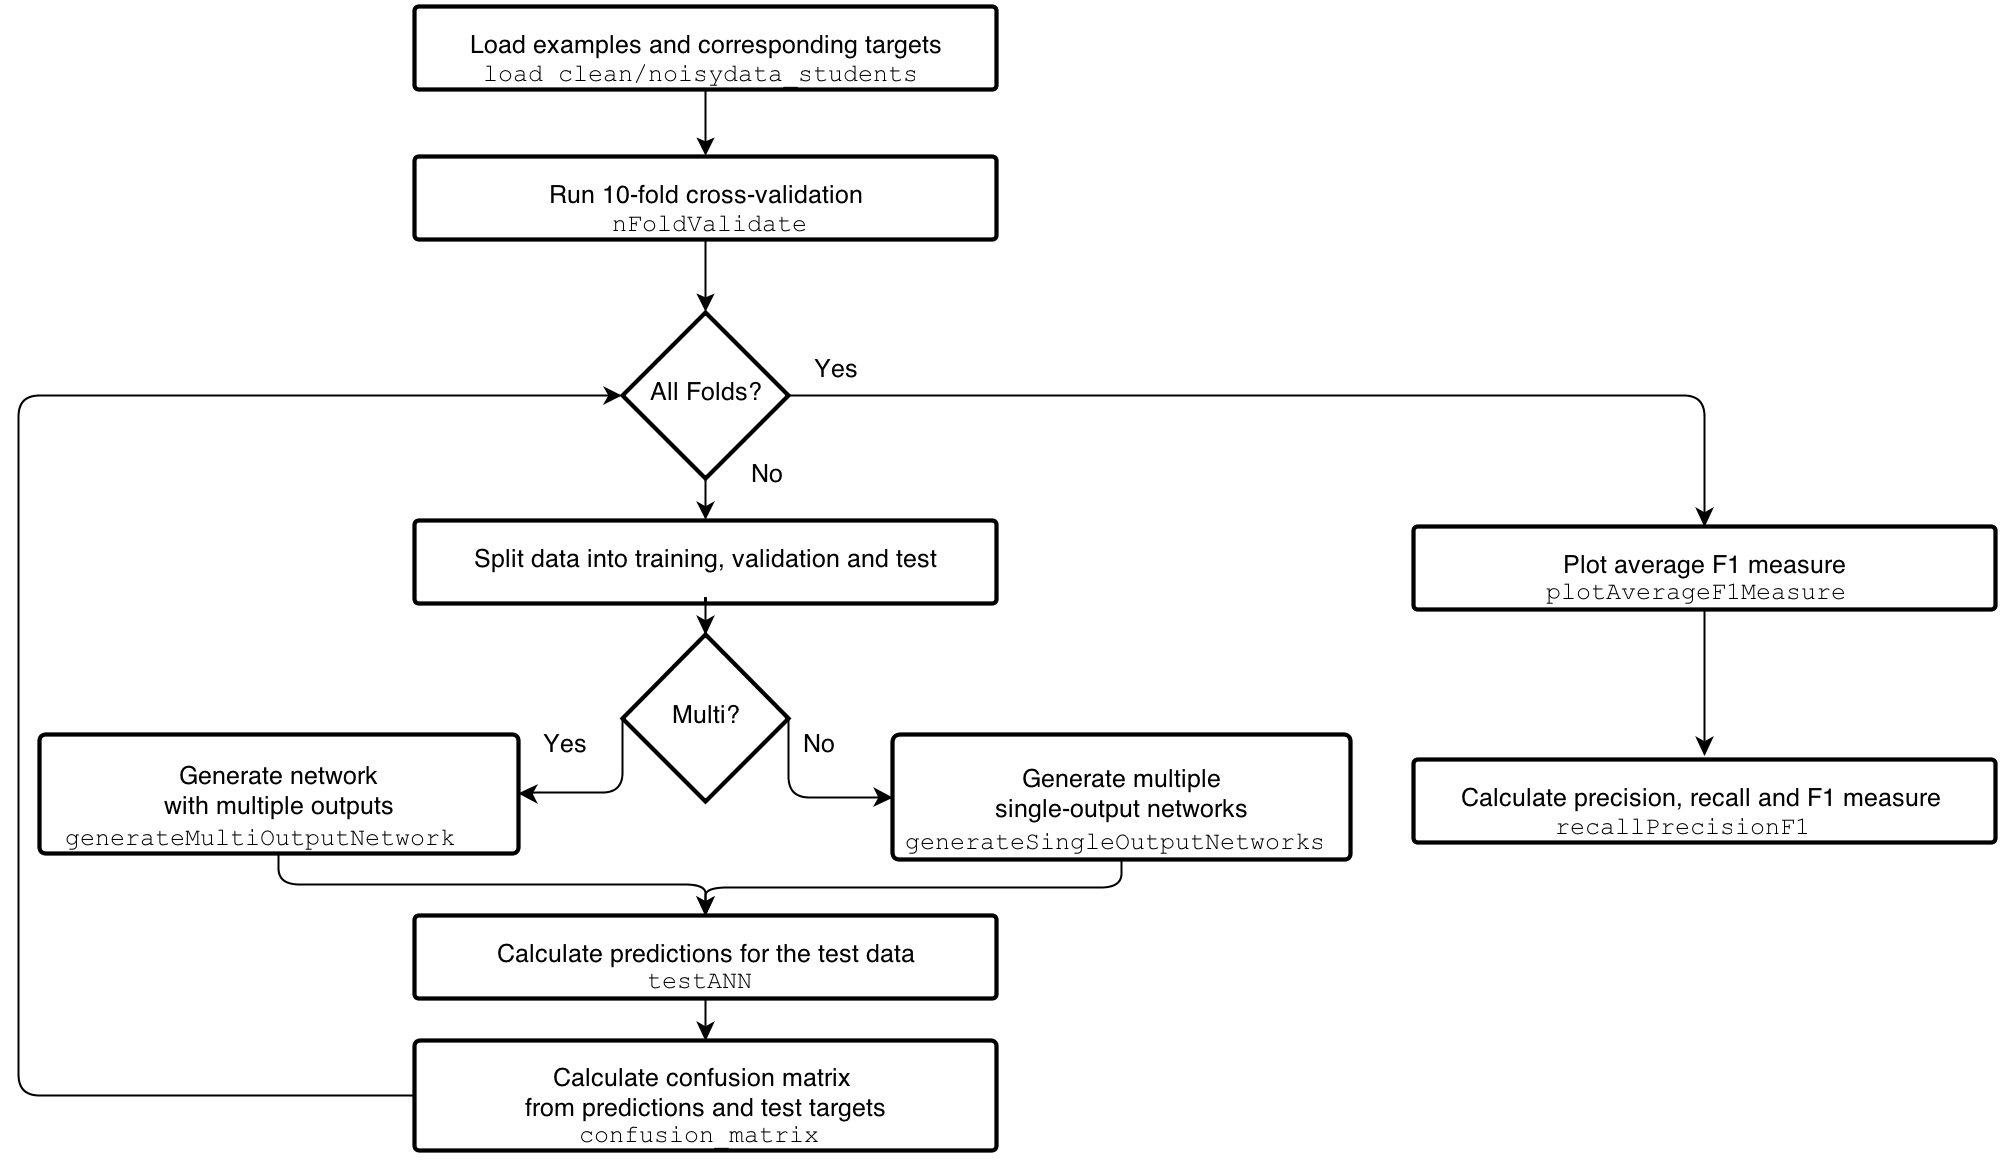
\includegraphics[width=1\columnwidth]{flowchart}
\caption{Code flowchart}
\label{flowchart}
\end{figure}

To perform the 10-fold cross-validation and plot the average $F_1$ measure for each fold (note that due to some random variation the result will be different from the one presented in this report):
\begin{lstlisting}
>> load cleandata_students.mat
>> singleOutputConfusionMatrix = nFoldValidate(x,y,10,'single');
>> multiOutputConfusionMatrix = nFoldValidate(x,y,10,'multi');
>> plotAverageF1Measure(singleOutputConfusionMatrix,multiOutputConfusionMatrix);
\end{lstlisting}

To generate a vector of predictions using the provided network:
\begin{lstlisting}
>> predictions = testANN(net,x); % 'net' can be either type of network, 'x' represents the examples
\end{lstlisting}

\clearpage

%----------------------------------------------------------------------------------------

\end{document}
